\chapter{最小生成树理论}
\label{chap:mst}

\section*{本章目标}
本章介绍生成树、最小生成树、最大生成树、Kruskal 算法、Prim 算法以及 cut property 和 cycle property。掌握这些结果后，\cref{chap:mst_recovery}中的拓扑恢复定理会变得非常自然。

\section{生成树与最小生成树}

\begin{definition}[生成树]
设 $G=(V,E)$ 是连通无向图。若 $T=(V,E_T)$ 是 $G$ 的子图且 $T$ 是树，则称 $T$ 是 $G$ 的生成树。
\end{definition}

给定边权函数 $c:E\to \R$，生成树 $T$ 的总权重为
\begin{equation}
  c(T)=\sum_{e\in E_T} c_e .
\end{equation}
最小生成树（minimum spanning tree, MST）是总权重最小的生成树：
\begin{equation}
  T^\star \in \argmin_{T\text{ 是 }G\text{ 的生成树}} c(T).
\end{equation}
若把目标改为最大化，则得到最大生成树。最大生成树常用于边概率解码：当 $c_{ij}$ 是边存在概率或相似度时，选择总相似度最大的放射状结构。

\begin{example}[距离与相似度的符号]
若 $c_{ij}$ 表示电气距离，边权越小越可信，应求 MST。若 $s_{ij}$ 表示“相邻概率”或相关相似度，边权越大越可信，应求最大生成树。最大生成树可等价地在权重 $c_{ij}=-s_{ij}$ 上求 MST。
\end{example}

\section{Kruskal 算法}

Kruskal 算法按边权从小到大扫描边，只加入不会形成环的边。

\begin{algorithm}[htbp]
  \caption{Kruskal 最小生成树算法}
  \label{alg:kruskal}
  \KwIn{连通无向图 $G=(V,E)$，边权 $c_e$}
  \KwOut{一棵 MST $T=(V,E_T)$}
  $E_T\leftarrow \varnothing$\;
  初始化并查集，使每个节点自成一个连通分量\;
  将 $E$ 按 $c_e$ 非降序排序\;
  \ForEach{$e=(u,v)\in E$ 按排序顺序}{
    \If{$u$ 与 $v$ 不在同一并查集分量}{
      $E_T\leftarrow E_T\cup\{e\}$\;
      合并 $u$ 与 $v$ 的分量\;
    }
    \If{$|E_T|=|V|-1$}{停止}
  }
  \KwRet{$T=(V,E_T)$}
\end{algorithm}

若使用排序和近似常数时间并查集，复杂度为
\begin{equation}
  O(|E|\log |E|).
\end{equation}
在完全图 $K_V$ 上，$|E|=O(|V|^2)$，排序可能成为主要开销。

\section{Prim 算法}

Prim 算法从一个初始节点出发，每次选择连接当前树与外部节点的最小边。

\begin{algorithm}[htbp]
  \caption{Prim 最小生成树算法}
  \label{alg:prim}
  \KwIn{连通无向图 $G=(V,E)$，边权 $c_e$，起点 $r$}
  \KwOut{一棵 MST $T=(V,E_T)$}
  $S\leftarrow\{r\}$，$E_T\leftarrow\varnothing$\;
  \While{$S\ne V$}{
    选择最小权跨割边 $e^\star=(u,v)$，其中 $u\in S,v\notin S$\;
    $E_T\leftarrow E_T\cup\{e^\star\}$，$S\leftarrow S\cup\{v\}$\;
  }
  \KwRet{$T=(V,E_T)$}
\end{algorithm}

使用二叉堆实现时，复杂度可达 $O(|E|\log |V|)$；对稠密图也可用邻接矩阵实现为 $O(|V|^2)$。在配电网拓扑恢复中，若距离矩阵已给出，完全图上 Prim 的矩阵实现很直接。

\section{割性质与环性质}

\begin{definition}[割与跨割边]
对非空真子集 $S\subset V$，割 $(S,V\setminus S)$ 的跨割边集合为
\begin{equation}
  \delta(S)=\{(u,v)\in E:u\in S,\ v\in V\setminus S\}.
\end{equation}
\end{definition}

\begin{theorem}[Cut property]
\label{thm:cut_property}
给定连通无向加权图 $G$。若边 $e$ 是某个割 $(S,V\setminus S)$ 上的唯一最小权跨割边，则 $e$ 属于每一棵 MST。
\end{theorem}

\begin{proof}
任取一棵 MST $T$。若 $e\in T$，结论成立。若 $e\notin T$，把 $e$ 加入 $T$ 会形成唯一环，该环必须还包含至少一条跨越同一割的边 $f$，否则从 $S$ 出发沿环经过 $e$ 后无法回到 $S$。由于 $e$ 是唯一最小跨割边，有 $c_e<c_f$。令
\begin{equation}
  T'=T\cup\{e\}\setminus\{f\}.
\end{equation}
则 $T'$ 仍为生成树，且 $c(T')=c(T)+c_e-c_f<c(T)$，与 $T$ 是 MST 矛盾。因此 $e\in T$。
\end{proof}

\begin{theorem}[Cycle property]
\label{thm:cycle_property}
若边 $e$ 是某个环上的唯一最大权边，则 $e$ 不属于任何 MST。
\end{theorem}

\begin{proof}
若某棵 MST $T$ 含 $e$，删除 $e$ 后 $T$ 分成两个连通分量。原环上除 $e$ 外必有一条边 $f$ 跨越这两个分量，否则环无法闭合。因为 $e$ 是唯一最大权边，$c_f<c_e$。用 $f$ 替换 $e$ 得到权重更小的生成树，矛盾。
\end{proof}

\section{唯一 MST 条件}

\begin{theorem}[互异边权推出 MST 唯一]
\label{thm:distinct_unique_mst}
若连通无向图 $G$ 的所有边权两两互异，则 MST 唯一。
\end{theorem}

\begin{proof}
反设存在两棵不同的 MST，记为 $T_1,T_2$。取对称差 $T_1\triangle T_2$ 中权重最小的边 $e$，不妨设 $e\in T_1\setminus T_2$。把 $e$ 加入 $T_2$ 得到唯一环 $C$。环 $C$ 中至少有一条边 $f\in T_2\setminus T_1$，否则 $T_1$ 本身含环。由于 $e$ 是对称差中最小边且边权互异，有 $c_e<c_f$。于是 $T_2\cup\{e\}\setminus\{f\}$ 是权重更小的生成树，矛盾。因此 MST 唯一。
\end{proof}

\section{一个配电网拓扑恢复例子}

\begin{figure}[htbp]
  \centering
  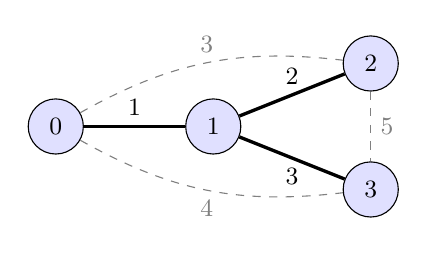
\begin{tikzpicture}[
  every node/.style={font=\small},
  bus/.style={circle,draw,fill=blue!12,minimum size=7mm}
]
\node[bus] (n0) at (0,0) {$0$};
\node[bus] (n1) at (2,0) {$1$};
\node[bus] (n2) at (4,0.8) {$2$};
\node[bus] (n3) at (4,-0.8) {$3$};
\draw[very thick] (n0)--node[above] {$1$} (n1);
\draw[very thick] (n1)--node[above] {$2$} (n2);
\draw[very thick] (n1)--node[below] {$3$} (n3);
\draw[dashed,gray] (n0) to[bend left=18] node[above,gray] {$3$} (n2);
\draw[dashed,gray] (n0) to[bend right=18] node[below,gray] {$4$} (n3);
\draw[dashed,gray] (n2)--node[right,gray] {$5$} (n3);
\end{tikzpicture}

  \caption{真实树距离上的 MST 恢复例子。完全图中未画出的边权为树上路径和，真实边是其基本割上的唯一最小边。}
  \label{fig:mst_example}
\end{figure}

\begin{example}[四节点馈线]
设真实配电树为 $0$--$1$--$2$ 和 $1$--$3$，边权分别为 $1,2,3$。由树路径和得到
\[
  d_{01}=1,\quad d_{12}=2,\quad d_{13}=3,\quad
  d_{02}=3,\quad d_{03}=4,\quad d_{23}=5.
\]
在完全图 $K_{\{0,1,2,3\}}$ 上以 $d_{ij}$ 为边权求 MST，Kruskal 首先选择 $(0,1)$，再选 $(1,2)$，再选 $(1,3)$，正好恢复真实树。这个例子是\cref{thm:additive_mst_recovery}的最小版本。
\end{example}

\section{本章小结}

MST 是在连通图上选择总权最小树的经典问题。Kruskal 从小边开始避免成环，Prim 从一个连通块开始反复跨割扩张。Cut property 说明唯一最小跨割边必进所有 MST；cycle property 说明唯一最大环边必不进 MST。边权互异是 MST 唯一的充分条件，但不是必要条件。下一章将利用 cut property 证明：若完整节点集上的距离是精确加性树距离，则 MST 可以恢复真实配电树。

\section*{思考题}
\begin{enumerate}
  \item 在一个三角形图中，边权分别为 $1,1,2$。MST 是否唯一？为什么？
  \item Kruskal 和 Prim 的输出是否一定相同？在什么条件下相同？
  \item 用 cycle property 解释为什么在距离图上很长的跨支路边不应进入 MST。
  \item 若边权是估计误差较大的电气距离，MST 会优先受哪些边影响？
\end{enumerate}
